\chapter{Introduction}

\section{Motivation}
The medical discipline of pathology is in a digital transformation. Instead of looking at tissue samples through the means of traditional light microscopes it now is possible to digitalize those samples. This digitalization is done with the help of a so called slide scanner. The result of such an operation is a\emph{whole slide image} (WHI)\nmc{WHI}{Whole Slide Image}\cite{Cornish13}. The digital nature of WHIs opens the door to the realm of image processesing and analysis which yields certain benefits, such as the use of image segmentation and registration methods to support the pathologist in his/her work.
\begin{figure}[ht]
	\begin{center}
		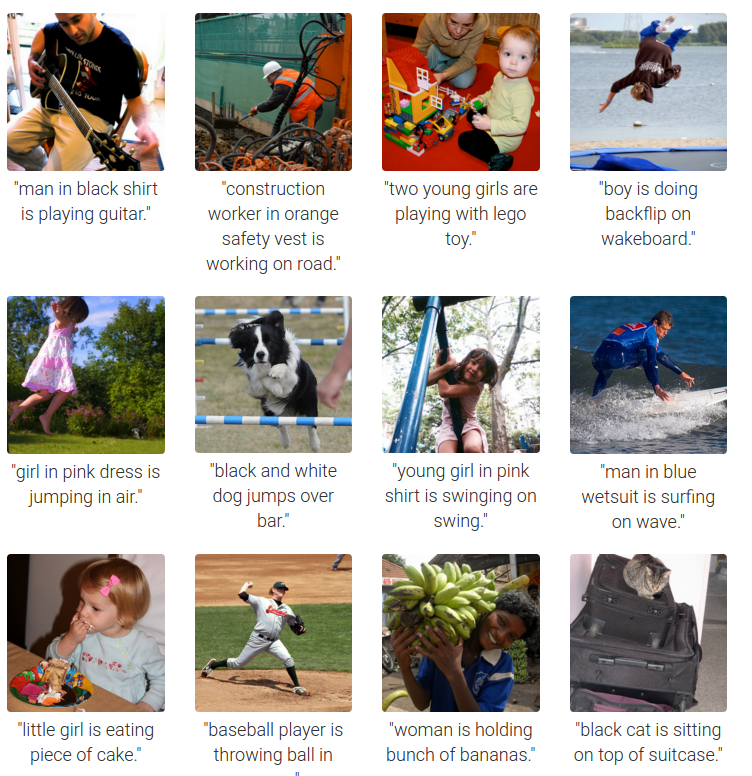
\includegraphics[scale=0.3]{img/deepVisual.png}
		\caption{Example results of the in \cite{Karpathy15} introduced model (source: http://cs.stanford.edu/people/karpathy/deepimagesent/}
		\label{fig:fig1.1}
	\end{center}
\end{figure}
A very promising area of image analysis are the so called \emph{neural networks}\footnote{See chapter 2.1.3}, which follow a machine learning approach. Their use, especially in the area of image classification and object recognition, made big breakthroughs possible in the recent past, e.g. Karpathy and Fei-Fei \cite{Karpathy15}, who created a neural network which is capable of describing an image or a scene with written text (see fig. 1.1 for some examples).

There is enormous potential in the use of neural networks in the digital pathology as well, but to transfer these algorithms and technologies, certain hindrances must be overcome. One of those hindrances is the need for proper training samples and an established ground truth\footnote{\emph{Ground truth} refers to a training sample whose outcome is known and validated as true.}. While generally there are huge amounts of WHIs, most of them won't be usable without further preparation as a training sample. One way of preparing them are annotations. These can be added to the WHIs, stored and later used for training.

Therefore the goal of this thesis is to give tools into the hands of pathologists to annotate whole slide images and save those annotations in such a way that they will be usable later in the combination with neural networks.


\section{Research Objective}
The objective of this thesis is the conceptualization and implementation of tools for WHIs, which allow for their annotation and a further usage in neural networks. As a requirement, the tools have to be implemented in the form of microservices\footnote{See chapter 2.1.2}, each one with their own short documentation, including instructions for installation, usage and some examplary use cases. To achieve this goal, the implementation of 3 microservices is necessary.

The first microservice needs to be capable of converting a given set of image formats into the so called \emph{Deep Zoom Image Format}\footnote{See chapter 2.1.1}. The supported image formats are \emph{.bif, .mrxs, .ndpi, .scn, .svs, .svslide, .tif, .tiff, .vms} and \emph{.vmu}, in accordance with the capabilities of the Openslide framework\cite{Goode13}.

The second microservices task is to give a tool at hand with which a pathologist will be able to annotate all those WHIs which were converted using the first microservice. Furthermore, the made annotations need to be persisted together with the highest resolution of the corresponding image.

The third microservice will be responsible for preparing the annotated WHIs for the further usage in neural networks. For that purpose the service needs to be capable of dividing a single annotated whole slide image into multiple tiles, with the choice of either using the whole image or just the annotated areas.


\section{About this thesis}
Apart from the \emph{Introduction}, there are 5 more chapters in this thesis.

\emph{Chapter 2 - Background} defines some terminoligy and the general, required process chain which are all necessary to understand further chapters of this thesis. Furthermore, 3 microservices will be introduced in short.

\emph{Chapter 3 - Methodology} gives an overview over the current state of research for each microservice, as well as best practices. 

\emph{Chapter 4 - Implementation} goes into further details about how each microservice is implemented and which software and frameworks were used for that.

\emph{Chapter 5 - Discussion} will introduce a measurement for each microservice to measure its success. It will discuss the test setup as well as list the results.

\emph{Chapter 6 - Conclusion} will interpret the Results from Chapter 5 and analyze them closer. Furthermore, it will give an idea of what steps are to be taken next in the future.